% !TEX root=../main.tex
\chapter{Methodology}
\renewcommand{\baselinestretch}{\mystretch}
\label{chap:method}
% \setlength{\parindent}{0pt}
\PARstart{T}{his} chapter will introduce the methodology of this project into two main aspects. One is to present pre-processing methods of audio data, including mel-spectrogram feature extraction, denoising method and data augmentation. The second aspect will introduce the architecture of CNN about activation function and different CNN layers. As to training CNN, the loss function and optimizer will be explained in the last section. 

\section{Mel-spectrogram Feature}
Spectrograms provide visual representations for people that can analyse the properties of audio data. As presented in Section 2.2, mel-spectrogram is an effective alternative for CNN as the input feature. However, the mel-spectrogram is based on the STFT which processed on discrete Fourier transform (DFT). It is expressed as $X_k=\sum ^{N-1}_{n=0}x_ne^{i2\pi \frac{kn}{N}}$, where $N$ coefficients are considered to represent the frequency value $X_k$. However, only several parts of audio we are interested since calls present a few seconds in most case. Therefore, separating the whole signal into shorter sections allows us to analyse the properties of particular points in time. By applying the window function to each segment, the STFT of signal can be obtained, which is expressed as
\begin{equation}
STFT\{ x_n\}(h,k)=X(h,k)=\sum_{n=0}^{N-1}x_{n+h}w_ne^{i2\pi \frac{kn}{N}}
\end{equation} 
where the length of window $h$ should be smaller than $N$. However, the represents of power spectrogram are non-uniform. Therefore, it is tough to extract informative features. By applying logarithm to power spectrogram can make representations more visual which is beneficial to analysis. Fig \ref{fig:powerlog} shows the difference of power spectrogram and spectrogram in the logarithm of example file '5AEF815A.wav'. Features are enhanced by taking the logarithm of the power spectrogram.\par 
\begin{figure}[htp]
     \begin{subfigure}[b]{0.5\linewidth}
         \centering
		  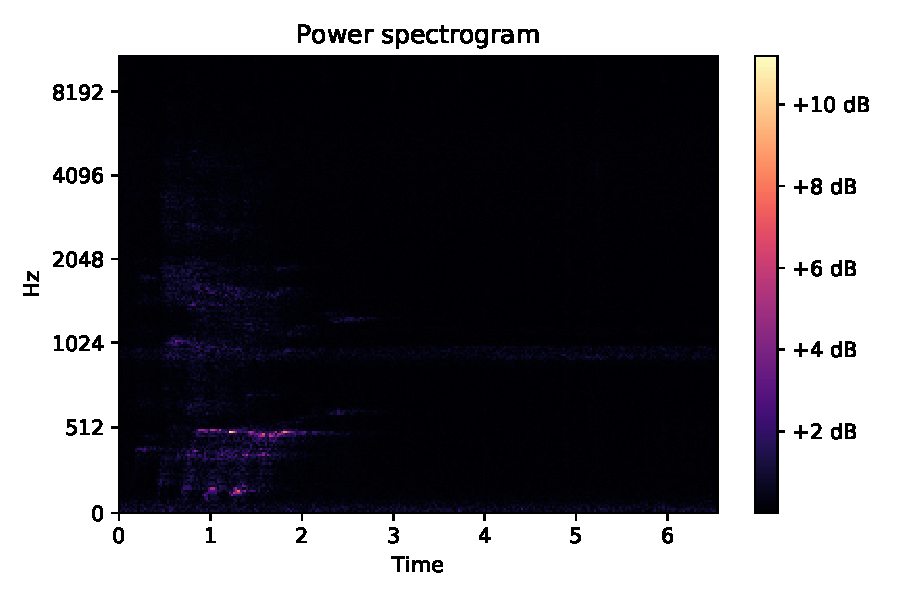
\includegraphics[scale=0.5]{Figs/chap3/power.pdf}
		  \caption{Power spectrogram}
     \end{subfigure}
     ~
     \begin{subfigure}[b]{0.5\linewidth}
         \centering
		  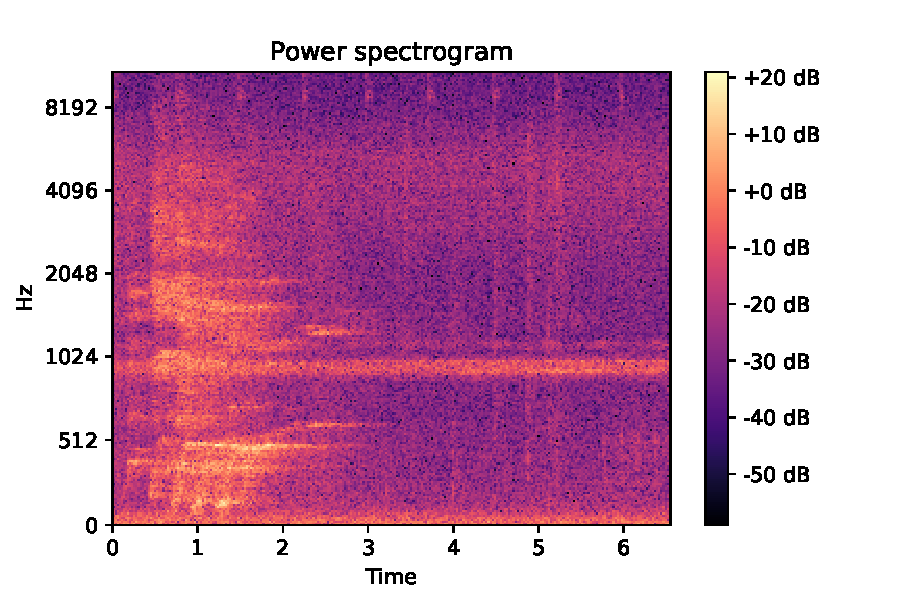
\includegraphics[scale=0.5]{Figs/chap3/logpower.pdf}
		  \caption{Log-scale spectrogram}
     \end{subfigure}
     \caption{Compare of power spectrogram and log-magnitude spectrogram (example file: 5AEF815A.wav)}
     \label{fig:powerlog}
\end{figure}
However, the STFT spectrogram is not the optimal extraction with the characteristic of linearity. By the inspiration of cochlea which can be considered as non-linear filters for the human sounds processing, the perceptual information can be introduced to the model. Specifically, emphasize the part of information which human listeners are sensitive and discriminative. After obtaining the short-time Fourier transform, the logarithm was applied to the magnitude to improve informative details. This process enhances the perceptual sensitive based on logarithmic-axis. Moreover, the frequency domain should be considered as well.

The mel-scale is one way to transform the original linear frequency into mel frequency. The mathematical approximation is 
\begin{align}
m&=2595\log_{10}(1+\frac {f}{700})\\
inverse: f&=700(10^{\frac{m}{2595}-1})
\end{align}
Therefore, the corresponding linear frequencies $f_i$ have equal perceptual distance by taking equally spaced mel-frequencies $m_i$. Fig~\ref{fig:melscale} (a) depicts the relationship between linear frequency in horizontal axis and the mel-frequency in vertical. However, other information will be degraded when using specific frequency $f_k$ during sampling the log-spectrogram. In other word, the transformation of mel-scale can be realized by applying filter bank to integrate the energy closed to the sample frequency $f_k$. 
\begin{equation}
u_k = \sum_{h=f_{k-1}+1}^{f_{k+1}-1} w_{k,h} |x_h|^2
\end{equation}
where $u_k$ is integrated energy in mel-spectrogram, $w_{k,h}$ is the weighted scalars and $x_h$ is the parts which close to sample frequency $f_k$. For the mel-scale, the weighted scalars are generally triangular function as shown in Fig~\ref{fig:melscale} (b). By combining weighted functions in non-linear spacing with 50\% overlapping, the log-spectrogram can be integrated and weighted.\par
\begin{figure}[htp]
     \begin{subfigure}[b]{0.5\linewidth}
         \centering
		  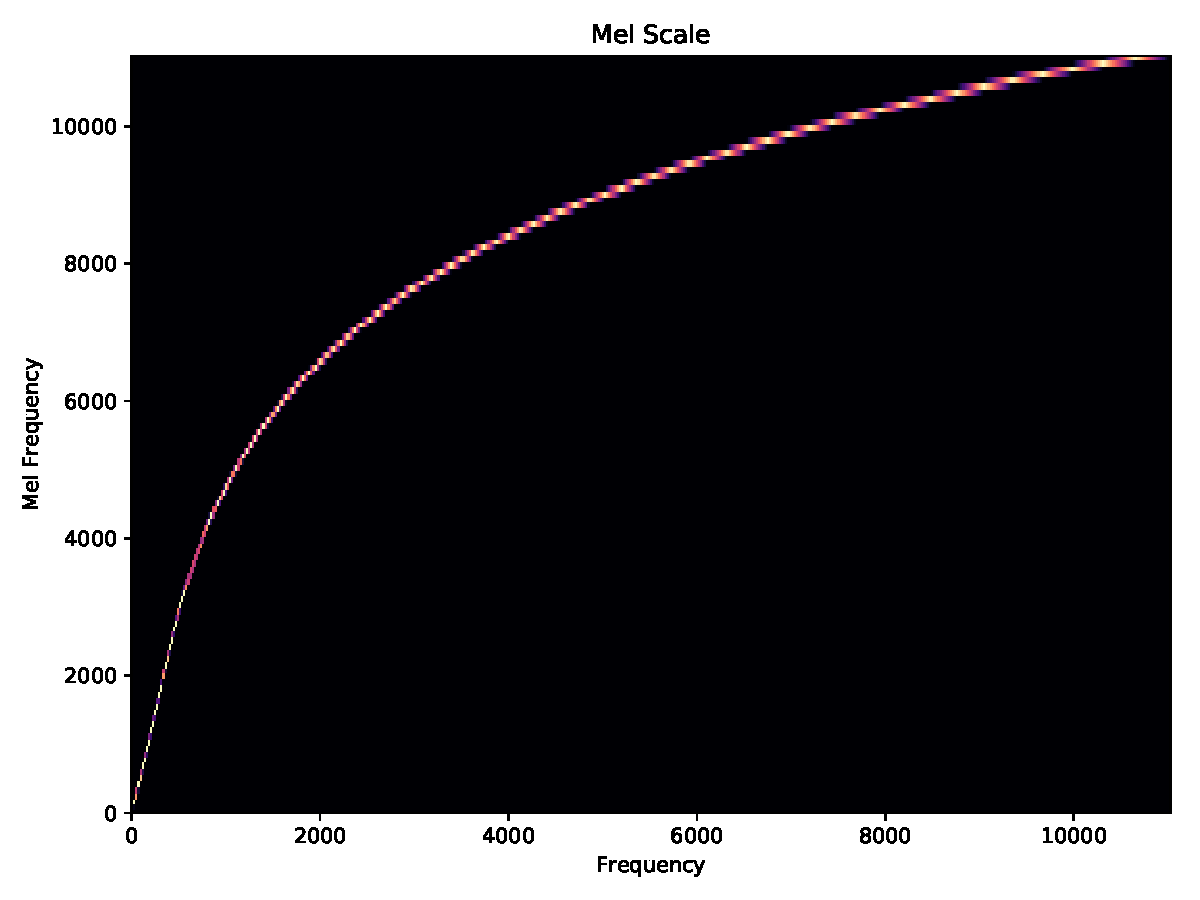
\includegraphics[scale=0.35]{Figs/chap3/mel_scale.pdf}
		  \caption{Mel scale function}
     \end{subfigure}
     ~
     \begin{subfigure}[b]{0.5\linewidth}
         \centering
		  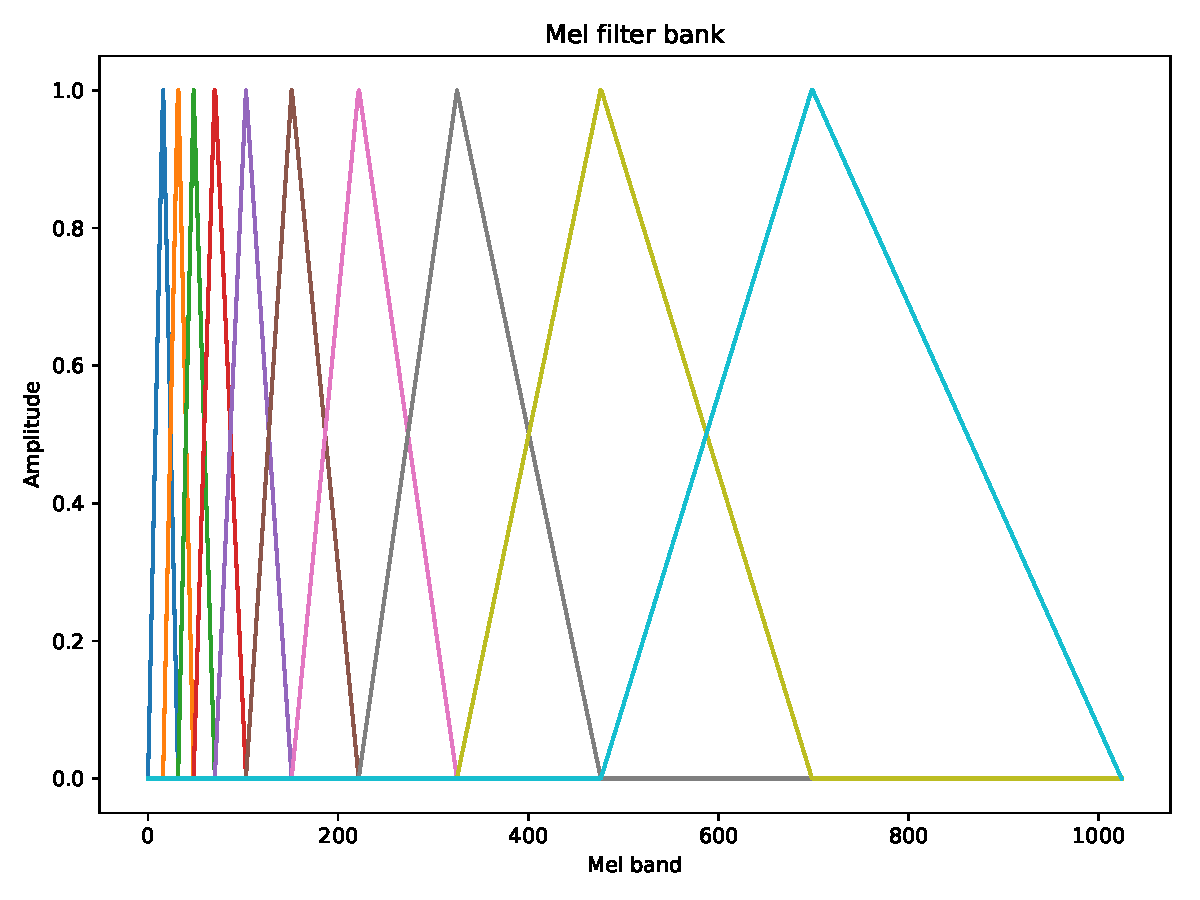
\includegraphics[scale=0.35]{Figs/chap3/mel_bank.pdf}
		  \caption{Mel filter bank with 10 mels}
     \end{subfigure}
     \caption{Transformation of frequency-to-mel and mel filter banks}
     \label{fig:melscale}
\end{figure}
By using triangular window above, the mel-spectrogram is obtained as show below. The mel-spectrogram contains more perceptual information which makes the presence of call more obvious. Therefore, using the mel-spectrogram as CNN model input can significant simulate how human make decisions. In addition, the MFCC can be calculated by taking discrete cosine transform (DCT) on log-scale mel-spectrogram. Due to MFCCs are not robust to additive noise, we chose mel-spectrogram as input feature.
\begin{figure}[htp]
\centering
  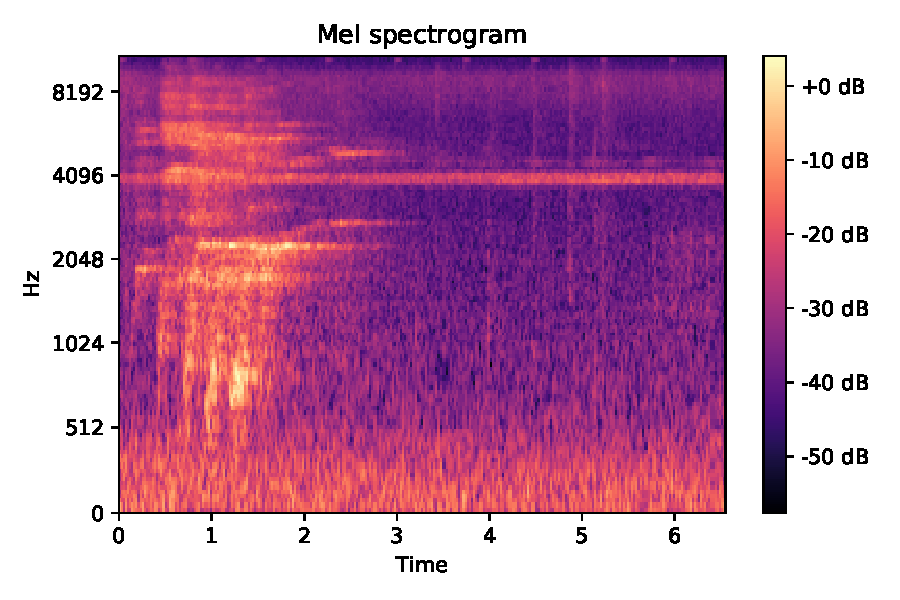
\includegraphics[scale=0.7]{Figs/chap3/mel_spec.pdf}
  \caption{Mel spectrogram}
 \label{fig:mel_spec}
\end{figure}
\section{Denoising Method}
The acoustic data of this project were recorded in the rainforest which caused complex and capricious environment. Thus, the signals of call presence were covered by large additive noise, resulting in inferior quality of audio. It is essential to apply denoising method to improve the signal noise ratio (SNR). We compared two performance of common denoising method, namely spectral subtraction~\cite{boll1979suppression} and MMSE-LSA estimator~\cite{ephraim1985speech}. First of all, as stated in their study, assume of the received noisy signal is 
\begin{equation}
y(t)=x(t)+n(t)
\end{equation}
where $x(t)$ is the desired signal and $n(t)$ is the noise. Thus, the equation above in frequency domain represents as
\begin{align}
Y(\omega)&=X(\omega))+N(\omega)\label{eq:spectrum}
\\
\notag
\end{align}
Only $y(t)$ and $Y(\omega)$ are known values. The objective of the denoising method is to reduce the noise interference without influencing the quality of the informative signal.
\subsection{Spectral Subtraction}
The aim of spectral subtraction is to estimate the power of noise based on the frequency domain $\hat N(\omega)$. Afterwards, the estimated spectrum of desired signal $\hat X(\omega)$ is obtained by
\begin{equation}
\hat X(\omega)=Y(\omega))- \hat N(\omega)
\label{sub-spec}
\end{equation}
Since the additive noise has the flat power along with the whole frequency band, the noise spectrum $\hat N(\omega)$ can be estimated as the expectation of noise spectrum $E\{|N(\omega)| \}$. This can be calculated by averaging parts where only noise recording presents at that time. The estimated noise spectrum can be denoted as 
\begin{equation}
\hat N(\omega)=E\{|N(\omega)| \}\cong |\bar N(\omega)|= \frac{1}{K}\sum_{i=0}^{K-1} |\bar N_i(\omega)|
\end{equation}
where $|\bar N_i(\omega)|$ is the i-th amplitude of K frames of noise. Therefore, the desired signal in frequency domain is calculated by the equation~\ref{sub-spec}. Hence, the time-series signal $x(t)$ is the inverse-Fourier transform of $\hat X(\omega)$.\par
The spectral subtraction estimator is a primary and effective method of noise reduction. The algorithm for estimating the noise spectrum is simple, resulting in less computing complexity. However, this approach assumes that the additive noise is wide-band and stationary, which does not always correspond to reality. Therefore, the reconstructed signal has a deviation to the theoretical desired signal in most cases. A large disturbance will be introduced due to the significant variations between estimated noise and actual noise As a consequence, the contributive information is distorted by the disturbance.
\par
Observing the original noisy mel-spectrogram in Fig~\ref{fig:mel_spec}, the presence of call is concentrated on the area of 512$\sim$3000 Hz frequency bands. It is notable that the uniform noise appears at 4096 Hz all the time. Fig~\ref{fig:spec_sub} demonstrates the  mel-spectrogram of reconstructed signal after using spectral subtraction estimator. Although the background was suppressed to a large extent, the estimator affects the quality of desired information as well. 
\subsection{MMSE Log-Spectral Amplitude Estimator}
As expressed in Eq~\ref{eq:spectrum}, the Fourier transform of noisy signal $Y(\omega)$, desired signal $X(\omega)$ and noise signal $N(\omega)$ can be expressed in complex form, which consists of amplitude spectral and phase spectral. Thus, for the $k$th frequency bin, the observed signal is expressed below:
\begin{align}
Y(\omega_k)&=X(\omega_k)+N(\omega_k)\\
R_k\exp(j\theta_k)&=A_k\exp(j\alpha_k)+N_k
\end{align}
where $R_k$, $A_k$ and $N_k$ are corresponding amplitude spectrums. Due to the noise is assumed as additive white Gaussian noise (AWGN), there is no phase spectrum of noise, resulting in . Hence, if we estimate the amplitude of desired signal $A_k$, the restored signal can be reconstructed by using phase of received signal.
\par
The MMSE-LSA estimator is an improved noise reduction method based on the MMSE short-time spectral amplitude~\cite{ephraim1985speech}. It has large difference of spectral subtraction which estimates the noise spectrum based on average frames. Nevertheless, the objective of MMSE-LSA is to minimise the mean-squared error between the actual log-amplitude of speech signal and log-amplitude of estimated signal, which can be expressed as 
\begin{align}
\arg\min_{\hat{A}_k}{\mathbb{E}\left[\left(\log A_k-\log\hat{A}_k\right)^2\vert y(t),0\leq t\leq T\right]}
\end{align} 
given the known condition of observed signal $\{ y(t), 0\leq t\leq T\}$. Obviously, the optimal solution for this problem is when the estimated amplitude equal to actual amplitude, leading to zero MMSE error. That is,
\begin{equation}
\hat A_k=\text{exp}\left\{\mathbb{E}\left[\ln A_k | Y_k\right]\right\}
\end{equation}
Based on the Gaussian model assumption, the term $\mathbb{E}\left[\ln A_k | Y_k\right]$ is calculated given by $Y_k$. Let $Z_k=\ln A_k$ and the moment function $\Phi_{Z_k|Y_k}(\mu)$ is
\begin{align}
	\Phi_{Z_k|Y_k}(\mu)&=\mathbb{E}\left\{\text{exp}(\mu Z_k) | Y_k\right\} \notag\\
	&= \mathbb{E}\left\{A_k^\mu | Y_k\right\} \label{eq:aa}
\end{align}
Thus, the aim is to calculate $\Phi_{Z_k|Y_k}(\mu)$ now and obtain $\mathbb{E}\left[\ln A_k | Y_k\right]$ by taking derivative of moment function at $\mu=0$. The moment function can be obtained from equation \ref{eq:aa}:
\begin{align}
\Phi_{Z_k|Y_k}(\mu)&=\mathbb{E}\left[A_k^\mu\vert Y_k\right] \\
&=\int_0^{\infty}\int_0^{2\pi}a_k^\mu p(a_k,\alpha_k\vert Y_k)d\alpha_k d a_k \\
&= \int_0^{\infty}\int_0^{2\pi}a_k^\mu \frac{p(a_k,\alpha_k,Y_k)}{p(Y_k)}d\alpha_k d a_k \\
&=\frac{ \int_0^{\infty}\int_0^{2\pi}a_k^\mu p(Y_k\vert a_k,\alpha_k) p(a_k,\alpha_k) d\alpha_k d a_k }{ \int_0^{\infty}\int_0^{2\pi} p(Y_k\vert a_k,\alpha_k) p(a_k,\alpha_k) d\alpha_k d a_k }
\end{align}
Since we assumed that each frequency bin confirms to Gaussian distribution, the probability was defined as following:
\begin{align}
p(Y_k\vert a_k,\alpha_k)&=\frac{1}{\pi\lambda_d (k)}\exp\left[ -\frac{1}{\lambda_d (k)}\vert Y_k - a_k e^{j\alpha_k} \vert^2 \right] \\
p(a_k,\alpha_k&)=\frac{1}{\pi\lambda_x (k)}\exp\left[-\frac{a_k^2}{\lambda_x (k)}\right]
\end{align}
where $\lambda_x (k)\triangleq \mathbb{E}\left[\vert X_k \vert ^2\right]=A_k^2 $ and $\lambda_d (k)\triangleq\mathbb{E}\left[\vert D_k \vert ^2\right]$. 
Based on the deduction in \cite{ephraim1985speech}, the amplitude of pure speech signal is calculated by
\begin{align}
\hat{A}_k=\frac{\xi_k}{1+\xi_k}\exp\left[\frac{1}{2}\int_{\upsilon_k}^{\infty}\frac{e^{-t}}{t}dt\right]R_k
\label{eq:magni}
\end{align}
and following parameters need to be estimated
\begin{align}
\upsilon_k\triangleq \frac{\xi_k}{1+\xi_k}\gamma_k;\quad
\xi_k\triangleq\frac{\lambda_x (k)}{\lambda_d (k)};\quad
\gamma_k\triangleq\frac{R_k^2}{\lambda_d (k)}
\label{eq:snr}
\end{align}
$\xi_k$ and $\gamma_k$ are considered as \textit{a prior} and \textit{a posterior} SNR respectively. The variance of noise can be updated by the voice activity detection (VAD) to detect the section without the presence of speech. Afterwards, \textit{a prior} SNR can be obtained by decision-directed method. Algorithm \ref{alg:mmse} demonstrates the procedure of MMSE-LSA estimator in Python realisation.\par
\begin{algorithm}
	\renewcommand{\algorithmicrequire}{\textbf{Input:}}
	\renewcommand{\algorithmicensure}{\textbf{Output:}}
	\caption{MMSE-LSA estimator for Python realisation}
	\label{alg:mmse}
	\begin{algorithmic}[1]
		\REQUIRE Noisy signal $y(t)$
		\ENSURE Enhanced signal $x(t)$
		\STATE Calculate the number of frames $N$ based on sampling frequency $f_s$
		\STATE Assume first 6 frames is noise/silence
		\FOR {k $\rightarrow$ 6}
		\STATE Windowing $y(t)$ in frame length $y(k)$
		\STATE FFT: y(k) $\rightarrow$ $Y(\omega_k)$
		\STATE Calculate variance of noise power $\lambda_d(k)$
		\ENDFOR 
		\FORALL{frames $k$ in $N$}
		\STATE FFT: y(k) $\rightarrow$ $Y(\omega_k)$
		\STATE Compute the power of noisy signal $R_k^2$
		\STATE Compute and limit a post SNR to avoid overflows $\gamma_k<40 dB$
		\STATE Calculate a priori SNR $\xi_k$ based on previous magnitude as shown in Eq.\ref{eq:snr}
		\STATE Estimate the magnitude of clean signal $X_k$ based on Eq.\ref{eq:magni}
		\ENDFOR
		\STATE IFFT: $X(\omega)\rightarrow x(t)$
		\STATE \textbf{return} $x(t)$
	\end{algorithmic}  
\end{algorithm}
Fig \ref{fig:logmmse} shows the mel-spectrogram after applying the MMSE-LSA estimator. Comparing with Fig \ref{fig:mel_spec}, the noise level was reduced to a large extent, presenting in lower magnitude of background. Moreover, the magnitude of call was enhanced, instead of attenuating in Fig \ref{fig:spec_sub}. Thus, the performance for MMSE-LSA method is outstanding than spectral subtraction in theoretically.
\begin{figure}[!htp]
     \begin{subfigure}[b]{0.5\linewidth}
         \centering
		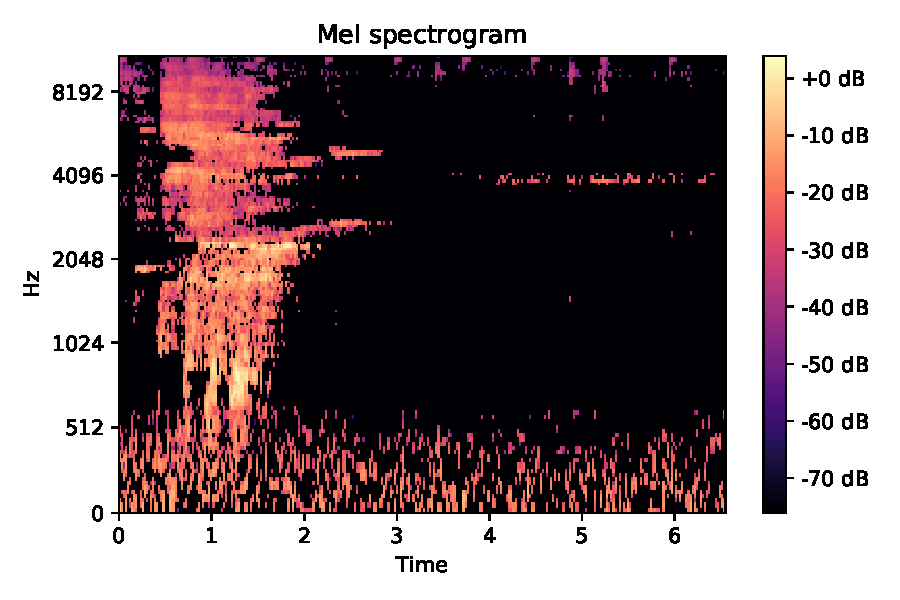
\includegraphics[scale=0.5]{Figs/chap3/sub_spec.pdf}
		\caption{spectral subtraction}
		\label{fig:spec_sub}
     \end{subfigure}
     ~
     \begin{subfigure}[b]{0.5\linewidth}
         \centering
		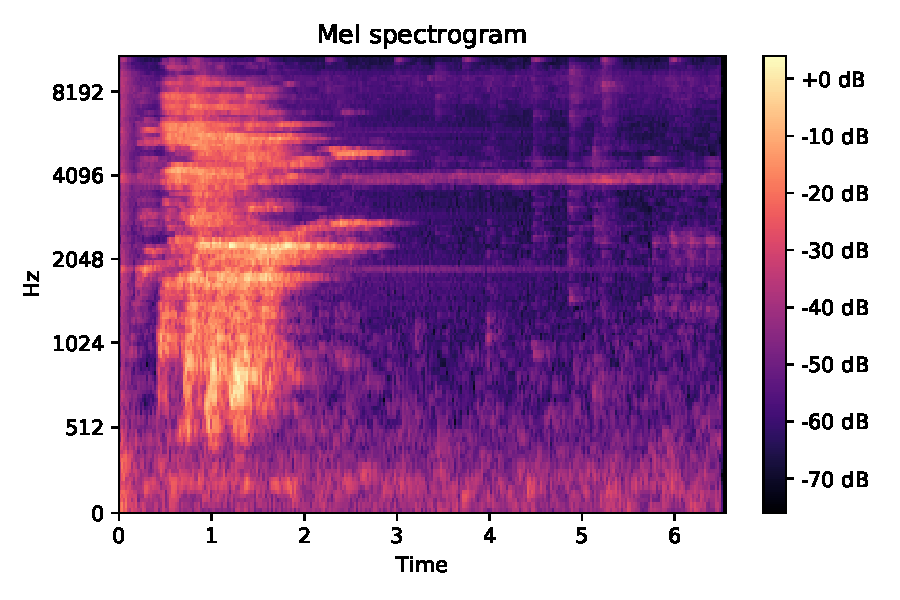
\includegraphics[scale=0.5]{Figs/chap3/logmmse.pdf}
		\caption{MMSE-LSA}
		\label{fig:logmmse}
     \end{subfigure}
  \caption{Mel spectrogram by using noise reduction methods}
  \label{Fig:denoise}
\end{figure}
\section{Data Augmentation}
For a CNN model, millions of weighted parameters need to be trained in hidden layers, which needs a mass of data to ensure the network fully trained. As to this project, since only 388 calls were collected for training, the data have to augment, avoiding the over-fitting problem. Moreover, it can improve the variation and generalisation of the model. I applied five common and effective augmentation methods to artificially generate data both on positives and negatives as similarly done by \cite{sprengel2016audio}. In addition, all augmentation methods are implemented in the time domain. For each augmentation, I randomly selected one of them to manipulate.
\begin{itemize}[leftmargin=*]
\item \textbf{Time-shift}\\
The audio signal is shifted in time with random position. Representing in the spectral domain is equivalent to vertically splinted the spectrogram into two segments. Time-shift will change the order of these two parts, resulting in sharp changes at joint. However, the model task is to detect the presence of whinny call which has less semantic relations among context. Furthermore, the total information is reserved. With this approach, the network has the ability to handle the irregular spectrogram and detect the call occurred at any time.
\item \textbf{Add noise}\\
Adding background noise is one of the most effective approaches to improve network performance. In section 3.2, I introduced the noise reduction method that enhances the speech region. However, the performance of model would pull down if only the denoised dataset was trained. At this circumstance, the model is biased with less generalisation, presenting in only recognizing noise-free clips. Hence, I added moderately amplitude of noise to the original file, combining with the noise reduced data to train. Moreover, I mixed part of negative samples to positive as well. 

\item\textbf{Pitch \& Speed}\\
As different augmentation methods were compared in \cite{schluter2015exploring}, the result showed that the pitch shift is significantly beneficial for improving. The pitch shift will change the frequency of sounds, resulting in vertical shift in the spectrogram. However, a large range of pitch shift will affect the biological features, which is not helpful for training. Time stretch will change the speed of the data. In order to maintain the same length of data, zeros were padded for speeding up and latter parts were removed for slow down mode. I applied a 5\% range of pitch shift and 10\% range of time stretch on raw data.
\item\textbf{Amplitude}\\
Changing amplitude is another way of augmentation. Since the version of data has large environmental noise, raising up the amplitude proved not a beneficial way. Hence, I emphasized to reduce dynamic amplitude with gain in $0.5\sim1.1$. 
\end{itemize}

\section{Design of CNN}
\subsection{Activation Functions}
In deep learning, the neuron is the basic unit which mimics the way of human brain transmitting and processing. The artificial neuron is a mathematical model that contains input, computing and output modules. With different connection ways between neurons, the neuronal network can realize a amount of tasks. As to a fully connection, each neuron will receive inputs from previous neurons and forward transmitting the processed result. This can be expressed in mathematical:
\begin{align}
\mathbf z^l &=\sigma(\mathbf w^l \mathbf a^{l-1}+b)
\end{align}
where $\mathbf w$ is the weight at current layer which need to be learned, $\mathbf a$ is the output of last layer, $\mathbf z$ is the neuron output, $\sigma$ is the activation function and $b$ is the scalar bias.

However, there is no activation function for perceptron model, whose final output is linear combinations of the input feature. This leads to a limited capability of network to deal with complex problem. Hence, the non-linearity activation functions are introduced so that the feature representation of DNN is powerful. By setting the number of neurons at each layer, the network can converge to arbitrary functions. Four common non-linear activation functions will be introduced as follows. In addition, Fig \ref{Fig:act} shows the output curves for each functions.
\begin{itemize}[leftmargin=*]
	\item \textbf{Sigmoid}\\
	The mathematical expression of sigmoid is denoted as
	\begin{equation}
		\sigma(x)=\frac{1}{1+e^{-x}}
	\end{equation}
	It is one of the non-linear activation functions. The advantage of sigmoid function that maps the infinite range value in limited range $(0, 1)$, which can be interpreted as the neuron firing rate. Thus, most of binary classification networks used sigmoid as the final output, indicating the positive or negative. However, two main shortcomings make sigmoid function less use in the hidden layer. Firstly, due to the nearly zero slope at large positive and negative regions, gradient vanishing problem appears at the process of back propagation, which makes network refuse to further learn. Moreover, the output of sigmoid is not zero-centred with all positive values. This causes the weight updating always in one direction (positive or negative). 
	\item \textbf{Tanh}\\
	As shown in Fig \ref{fig:sig}, the tanh function has the similarity of the sigmoid function, which can be expressed as
	\begin{equation}
		\tanh(x)=\frac{e^{x}-e^{-x}}{e^{x}+e^{-x}}=2*sigmoid(2x)-1
	\end{equation}
	Although the tanh solved the zero-centred problem of sigmoid, gradient vanishment is still an issue for tanh during back propagation.
	\item \textbf{ReLU \& eLU}\\
	ReLU is the short term of rectified linear unit and the expression is denoted as
	\begin{equation}
	A(x) = max(0,x)	
	\end{equation}
	Although it is simple in mathematics, many of studies prove the outstanding performance of ReLU \cite{maas2013rectifier}. Firstly, the computational cost is quite small (only need to judge the input if is positive). Therefore, it converges faster than tanh and sigmoid function. Additionally, it overcomes the gradient vanishing problem in the positive region. However, the output of ReLU is still not zero-centred. Due to forced rectifying to zero for negatives, the dead ReLU problem appears for some neurons which will never be activated. For solving this problem, leaky ReLU and eLU are introduced, changing the function in negative part.\\
	Exponential Linear Units, namely eLU, has all distinctions of ReLU. The negative part is modified into an exponential function, which is robust for noise. The average output of eLU is near zero without dead neuron problem. Thus, it should be outstanding compared with ReLU function, in spite of increasing computation. Nevertheless, few experiments demonstrated that the performance of eLU is better. Hence, I selected ReLU function applied in the design of CNN architecture.
\end{itemize}
\begin{figure}[!htp]
     \begin{subfigure}[b]{0.5\linewidth}
         \centering
		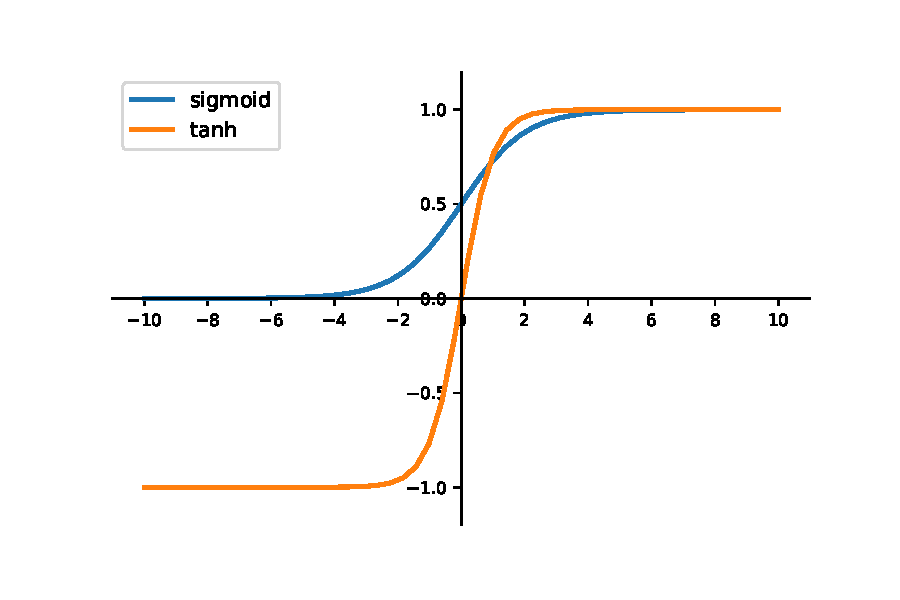
\includegraphics[scale=0.5]{Figs/chap3/act1.pdf}
		\caption{Sigmoid and tanh}
		\label{fig:sig}
     \end{subfigure}
     ~
     \begin{subfigure}[b]{0.5\linewidth}
         \centering
		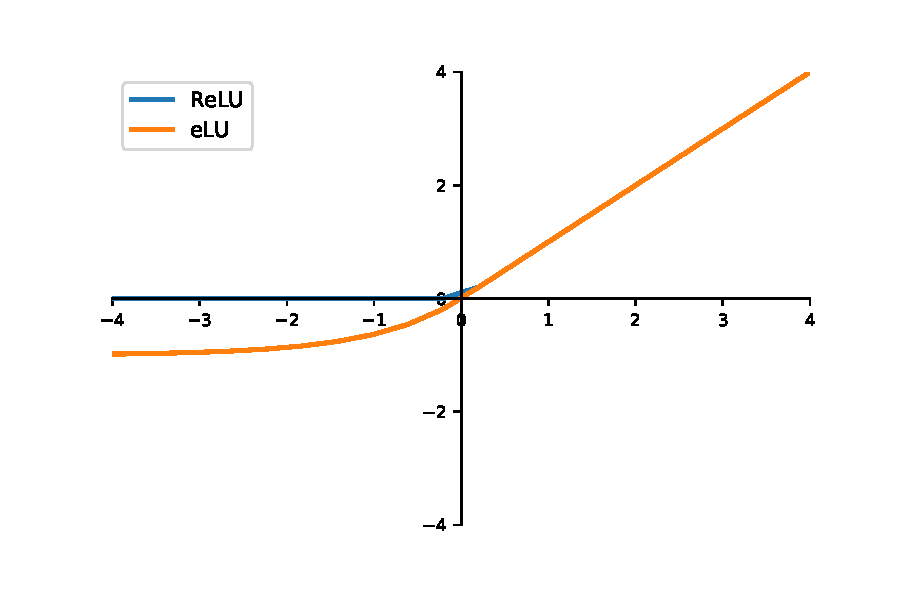
\includegraphics[scale=0.5]{Figs/chap3/act2.pdf}
		\caption{ReLU and eLU}
		\label{fig:relu}
     \end{subfigure}
  \caption{Different activation functions output curve}
  \label{Fig:act}
\end{figure}
\subsection{Layers of CNN}
The network is designed by a combination of different layers. In general, there are three main layers for CNN architecture, connecting in hierarchical order.
\begin{itemize}[leftmargin=*]
	\item\textbf{Convolutional layers}\\
	The convolutional layer is the principal layer of CNN, which is used to extract features. It is performed by applying certain size filters to the input, accumulating masked values to get one output. With different weights in filters, the output can learn diverse features. Fig \ref{fig:filter} depicts the operation of filter convolution. For example, applying a $5\times5$ filter to the input will obtain one individual output. However, $5\times5$ size filter can be replaced by using two successive $3\times3$ filters, resulting in the same shape of output. This is the basic operation of VGG Network which makes network deeper.
	\begin{figure}[htp]
	\centering
	  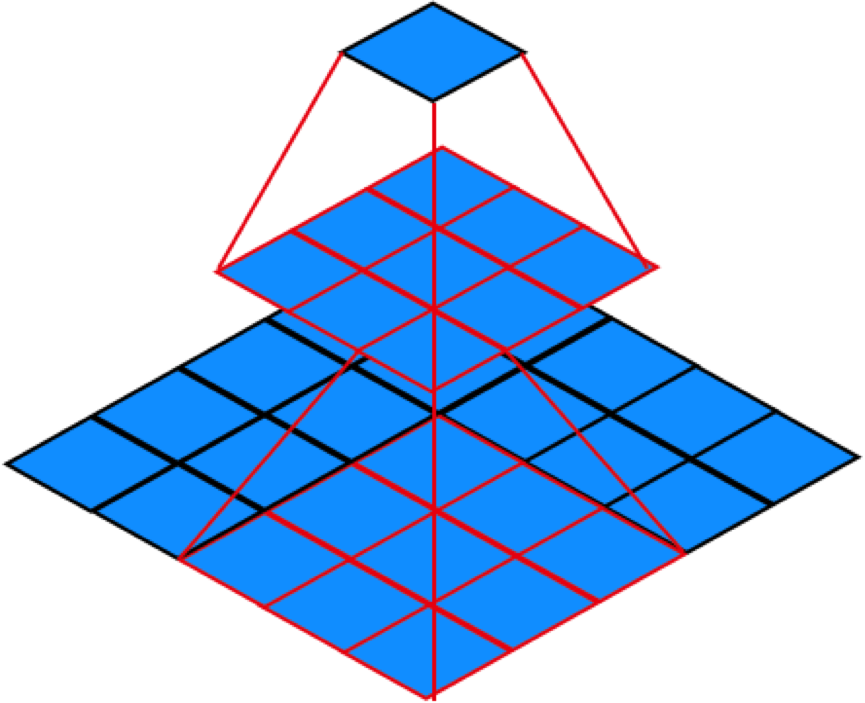
\includegraphics[scale=0.5]{Figs/chap3/vggfilter.png}
	  \caption{visualisation of convolutional filters in VGGNet}
	 \label{fig:filter}
	\end{figure}
	\item\textbf{Pooling layers}\\
	Pooling layers are normally following with convolutional layers. There are two aims of pooling that one is to reduce the dimension of parameters after convolution. On the other, the extracted features are compressed by selecting significant feature. In this project, maximum pooling layers were used to extract the maximum value in the corresponding region. It is an important procedure to prevent network over-fitting. Meanwhile, the computation speed is accelerated due to reducing feature dimension.
	\item\textbf{Fully-Connected (Dense) layers}\\
	Fully-connected or dense layers are the final section of the network. It firstly transforms the matrix into vector representation via convolving the matrix of each neuron. With FC layers, all neurons in current layer are connected to the next layer. Hence, features are combined in order to fit the distribution of data. Softmax or sigmoid activation functions are applied at the end as the classification output of the model.
\end{itemize}
\section{Model Training}
\subsection{Loss Functions and Optimizer}
Loss function plays an important role in training network and assists in back propagation. For a time step, the input data will pass through the CNN network and obtain a prediction at the end layer. A loss is generated to measure the divergence between the actual label $y$ and the prediction $\hat y$. As to one epoch, all training samples losses of each time step are summed together to calculate the back propagation step. The expression is 
\begin{equation}
\boldsymbol{\mathcal{L}}(\boldsymbol{\theta})=\frac{1}{n}\sum_{i=1}^{n}L\big(y^{(i)},f(\mathbf{x}^{(i)},\boldsymbol{\theta})\big)
\end{equation}
where $\mathbf{x}$ and $\boldsymbol{\theta}$ are training samples and learning features respectively, $f(\cdot)$ represents the model output. There are several different loss functions, dealing with various tasks. Cross entropy (CE) is one of extensively used function with outstanding performance, especially in classification problem \cite{simard2003best}. In our case, the learning problem is a binary classification task which needs model to detect the positives and negatives. Hence, binary cross-entropy was applied for this work. The mathematical expression is shown below,
\begin{equation}
\boldsymbol{\mathcal{L}}=-\frac{1}{n}\sum_{i=1}^{n}\big[y^{(i)}\log(\hat{y}^{(i)})+(1-y^{(i)})\log(1-\hat{y}^{(i)})\big]
\label{eq:loss}
\end{equation}
The former term measures the positive prediction loss and the latter is for negative. Thus, if the true label is positive/negative (1/0) while the prediction is far different from the actual label, a large loss is introduced. Due to only logarithm and summation operation, the gradient can be computed rapidly compared with MSE loss function. 

Once we defined the loss function, the optimiser needs to be chose for converging up to global optimum. An outstanding optimiser has the capability of not only fast convergence but also maintaining model recall. Adaptive moment estimation (Adam) optimiser \cite{kingma2014adam} computes both first and second-order moment to gradient descent. Since the mean and uncentered variance of the gradient are estimated, the Adam optimiser can adaptively adjust learning momentum, resulting in fast convergence speed compared with other gradient descent algorithms. As shown in practical experiments \cite{ruder2016overview}, Adam optimiser has an impressive performance. Thus, we apply Adam optimiser to reduce loss in Eq \ref{eq:loss} with default values of $\beta_1$, $\beta_2$ and $\epsilon$. The learning rate was set to $10^{-5}$. 
\subsection{Hyperparameter Tuning}
After constructing the network, the model needs to be trained with appropriate parameters. The metrics are significant for evaluating the performance of model, which concentrates on targets of true positives (TP), false positives (FP), true negatives (TN) and false negatives (FN). Based on these targets, four different metrics are used to evaluate the network, namely accuracy, precision, recall and F1 score. Accuracy is the general metric to assess the performance. Precision represents how many true positives were detected among positive predictions, which is the ratio of TP with the summation of TP and FP. Recall evaluates how many positives can be mined by model, which is TP/(TP+FN). F1 score is the weighted combination of recall and precision. Hence, the model can be considered as optimum whichever achieves the expressive accuracy and F1 score.

Even though we use the fixed dataset to train the model, the eventual objective is to reduce generalisation error as much as possible. Thus, tuning network is an important part of training. As to tuning hyperparameters, the validation dataset is applied to evaluate performance during model training. It differs from test dataset that when the model is fine-tuned, the validation set will add to the training set for the final training. By observing metrics of the validation set, the hyperparameters can be tuned. Due to the limited GPUs and the size of dataset, the batch size is set to 16. 
\begin{itemize}[leftmargin=*]
	\item \textbf{Training Epoch}\\
	For one time step, the CNN model will only concentrate on the batch size of data. When all training data are learned forward and updated backwards once, the CNN network is trained for one epoch. Thus, with large training epochs, the model could learn features multiple times. However, the model is insufficiently trained if epoch is too small. Hence, the threshold needs to be determined. By excessively set epoch to make model over-fitting on purpose, the appropriate threshold is easy obtained. Fig \ref{Fig:learning} demonstrates the training and validation loss with 100 epochs. After 50 epochs, the validation loss decreases significantly slowly compared with training loss. The difference between validation and training becomes larger, which caused the over-fitting problem on training data. Therefore, the epoch is set to 50.
	\begin{figure}[htp]
	\centering
	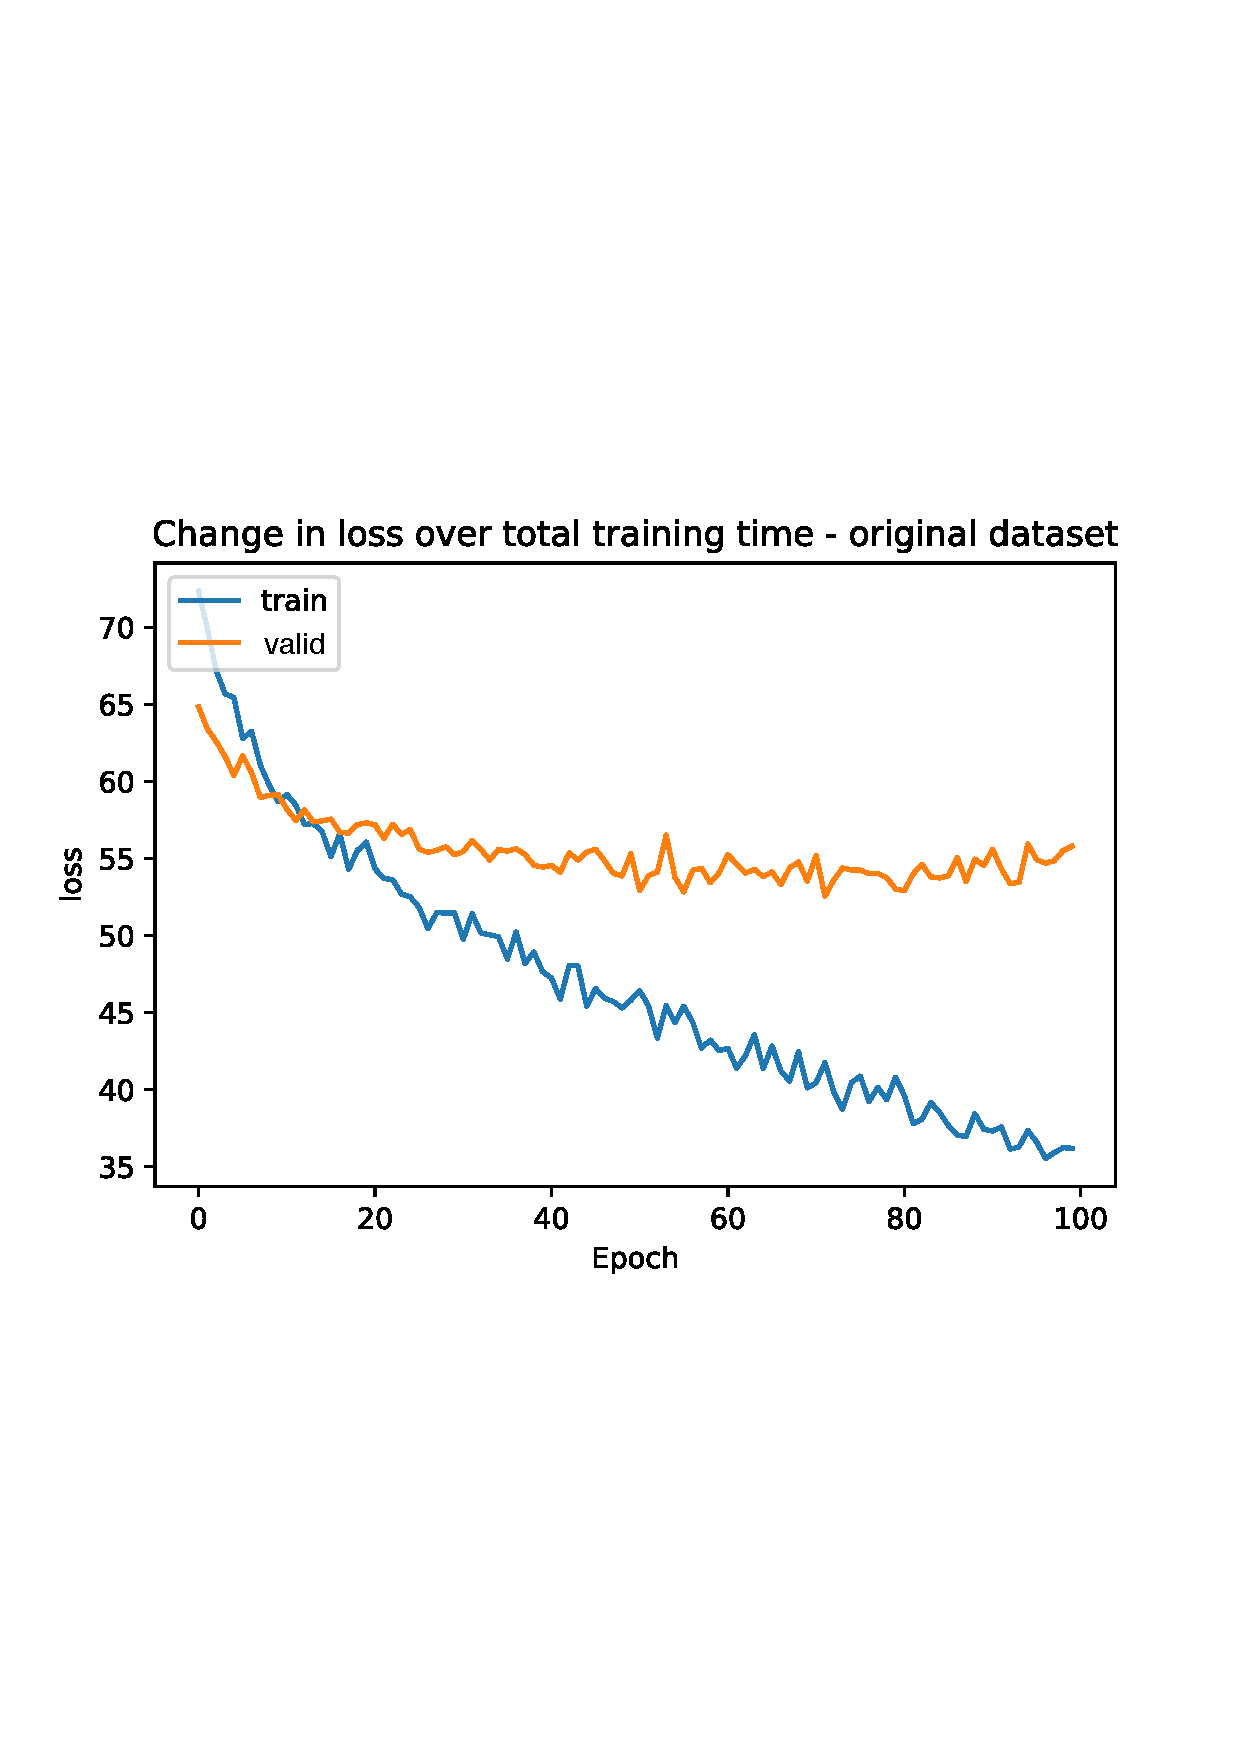
\includegraphics[scale=0.45]{Figs/chap3/e100.pdf}
	\caption{Training and validation loss curves of 100 training epochs}
	\label{fig:epoch}
	\end{figure}
	\item \textbf{Learning rate}\\
	Learning rate of the optimiser is another parameter that affects the loss. Although a large learning rate can rapidly converge to the optimum, it will result in the zigzag problem, oscillating near the global optimum. Fig \ref{Fig:learning} depicts the loss of learning rate in $10^{-4}$ and $10^{-5}$. The model appears over-fitting problem after 20 epochs in Fig \ref{fig:10-4}, presenting in an increasing trend of validation loss. When reducing learning rate 10 times, the loss slightly falling down without over-fitting. Thus, the learning rate is determined as $10^{-5}$, even if the final loss is large.  
	\begin{figure}[htp]
     \begin{subfigure}[b]{0.5\linewidth}
         \centering
		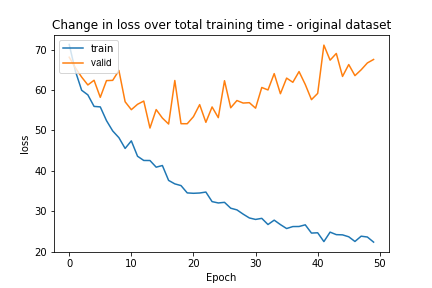
\includegraphics[scale=0.5]{Figs/chap3/10-4.png}
		\caption{learning rate=$10^{-4}$}
		\label{fig:10-4}
     \end{subfigure}
     ~
     \begin{subfigure}[b]{0.5\linewidth}
         \centering
		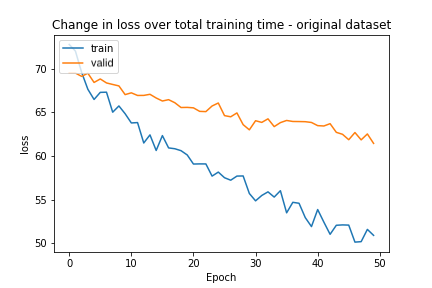
\includegraphics[scale=0.5]{Figs/chap3/10-5.png}
		\caption{learning rate=$10^{-5}$}
		\label{fig:10-5}
     \end{subfigure}
  \caption{Training and validation loss curves of varying learning rate}
  \label{Fig:learning}
\end{figure}
\end{itemize}

\subsection{Hard Negative Mining}
In this project, the negative data consists of other animal calls, environmental sounds and white noise. Since the negative examples are relatively effortless to obtain compared to rare positive calls, the number of negative examples is more than that of positives. Therefore, the variance and quality of negatives have large differences. For example, the white noise is significantly easy to be classified while other animal calls are not. As to further improving the model performance, hard negative mining approach can be applied to model training. Experiments proved this method is effective on objective detection tasks by SVM \cite{felzenszwalb2009object} and region-CNN (R-CNN) \cite{girshick2014rich}. They firstly used random bounding boxes to train the model. The boxes without overlapping with positives are called easy negatives and those with part of targets are difficult to be classified. Subsequently, these hard negatives were selected to form a new hard-negative dataset and retrain the model. After repeating several times, the performance of model is improved to a large extent. 
	\begin{figure}[!htp]
	\hskip-1.5em
     \begin{subfigure}[b]{0.5\linewidth}
         \centering
		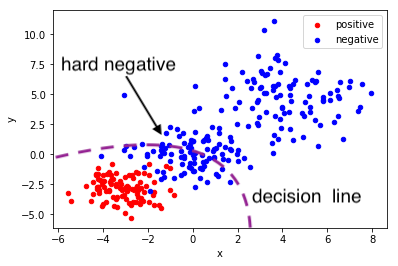
\includegraphics[scale=0.55]{Figs/chap3/pn.png}
		\caption{original data}
		\label{fig:pn}
     \end{subfigure}
     ~
     \begin{subfigure}[b]{0.5\linewidth}
         \centering
		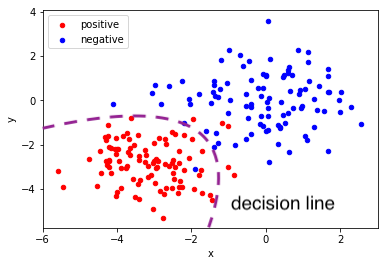
\includegraphics[scale=0.55]{Figs/chap3/hnm.png}
		\caption{hard negatives}
		\label{fig:hn}
     \end{subfigure}
  \caption{Hard negative mining examples in two-dimension}
  \label{Fig:hnm}
\end{figure}

Fig \ref{Fig:hnm} demonstrates the principle of hard negative mining in two-dimensional representation. The negatives with near distance to positives are hard samples to be classified. Thus, the decision boundary is influenced by the easy negatives for first trained.  A large amount of negatives are classified as positives. When applying hard negative mining method, only hard samples are selected for the second train. Thus, the decision boundary is more distinct compared with the first training model, resulting in outstanding accuracy. As to this work, the hard negative mining only applied once to train the model totally twice.

